\documentclass[a4paper]{article}
\usepackage[margin=3.9cm]{geometry}
\usepackage{amsmath}
\usepackage{amssymb}
\usepackage{xcolor}
\usepackage{amsthm}
\usepackage{dsfont}
\usepackage{graphicx}
\usepackage{hyperref}
\usepackage{datetime}
\usepackage{outlines}
\usepackage{float}
\usepackage{booktabs}
\usepackage{enumitem}


\definecolor{fgcolor}{rgb}{0.345, 0.345, 0.345}
\newcommand{\hlnum}[1]{\textcolor[rgb]{0.686,0.059,0.569}{#1}}%
\newcommand{\hlstr}[1]{\textcolor[rgb]{0.192,0.494,0.8}{#1}}%
\newcommand{\hlcom}[1]{\textcolor[rgb]{0.678,0.584,0.686}{\textit{#1}}}%
\newcommand{\hlopt}[1]{\textcolor[rgb]{0,0,0}{#1}}%
\newcommand{\hlstd}[1]{\textcolor[rgb]{0.345,0.345,0.345}{#1}}%
\newcommand{\hlkwa}[1]{\textcolor[rgb]{0.161,0.373,0.58}{\textbf{#1}}}%
\newcommand{\hlkwb}[1]{\textcolor[rgb]{0.69,0.353,0.396}{#1}}%
\newcommand{\hlkwc}[1]{\textcolor[rgb]{0.333,0.667,0.333}{#1}}%
\newcommand{\hlkwd}[1]{\textcolor[rgb]{0.737,0.353,0.396}{\textbf{#1}}}%
\let\hlipl\hlkwb

\usepackage{framed}
\makeatletter
\newenvironment{kframe}{%
 \def\at@end@of@kframe{}%
 \ifinner\ifhmode%
  \def\at@end@of@kframe{\end{minipage}}%
  \begin{minipage}{\columnwidth}%
 \fi\fi%
 \def\FrameCommand##1{\hskip\@totalleftmargin \hskip-\fboxsep
 \colorbox{shadecolor}{##1}\hskip-\fboxsep
     % There is no \\@totalrightmargin, so:
     \hskip-\linewidth \hskip-\@totalleftmargin \hskip\columnwidth}%
 \MakeFramed {\advance\hsize-\width
   \@totalleftmargin\z@ \linewidth\hsize
   \@setminipage}}%
 {\par\unskip\endMakeFramed%
 \at@end@of@kframe}
\makeatother

\definecolor{shadecolor}{rgb}{.97, .97, .97}
\definecolor{messagecolor}{rgb}{0, 0, 0}
\definecolor{warningcolor}{rgb}{1, 0, 1}
\definecolor{errorcolor}{rgb}{1, 0, 0}
\newenvironment{knitrout}{}{} % an empty environment to be redefined in TeX


% code highlighting
\usepackage{minted}
\usepackage{xpatch}
\newminted[cminted]{python}{fontsize=\small}
\xpretocmd{\cminted}{\RecustomVerbatimEnvironment{Verbatim}{BVerbatim}{}}{}{}

% link coloring
%\hypersetup{
%    colorlinks,
%    linkcolor={red!80!black},
%    citecolor={green!60!black},
%    urlcolor={blue!80!black}
%}

% concatenation symbol (c.f. ++ in Haskell)
\newcommand\mdoubleplus{\mathbin{+\mkern-10mu+}}

% end of proof symbol
\newcommand{\newmarkedtheorem}[1]{%
  \newenvironment{#1}
    {\pushQED{\qed}\csname inner@#1\endcsname}
    {\popQED\csname endinner@#1\endcsname}%
  \newtheorem{inner@#1}%
}

\theoremstyle{definition}
%\newtheorem{eg}{Example}[section]
\newmarkedtheorem{eg}{Example}[section]
\newtheorem{observation}{Observation}[section]
\newtheorem{define}{Definition}[section]
\theoremstyle{plain}
\newtheorem{proposition}{Proposition}
\newtheorem{lemma}{Lemma}
\newtheorem{corollary}{Corollary}
\newtheorem{theorem}{Theorem}[section]
\newtheorem{assump}{Assumption}[section]
\newtheorem{remark}{Remark}[section]

\newdateformat{monthyeardate}{\monthname[\THEMONTH] \THEYEAR}

\author{Jeroen van Riel}
\date{\monthyeardate\today}
\title{Offline Trajectory Optimization of Autonomous Vehicles in a Network of Intersections}

\begin{document}

\maketitle

\tableofcontents

\section{Trajectories in networks}

\begin{figure}
  \centering
  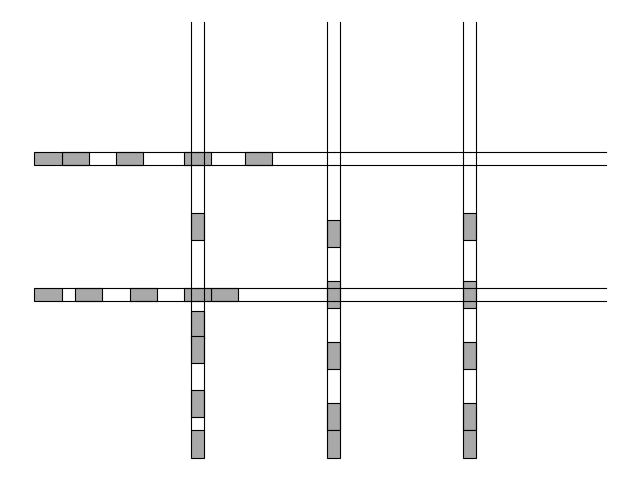
\includegraphics[width=0.55\textwidth]{figures/state_example.png}
  \caption{Illustration of some grid-like network of intersections with vehicles
    drawn as grey rectangles. There are five vehicle routes: two from east to
    west and three from south to north. Turning at intersections is not
    allowed.}\label{fig:network_illustration}
\end{figure}

We now extend the single intersection model to a network of intersections
without turning routes, illustrated in Figure~\ref{fig:network_illustration}.
% network definition
We define a directed graph $(V,E)$ with nodes $V$ and arcs $E$, representing the
possible paths that vehicles can follow. Nodes of in-degree at least two are
called \textit{intersections}. Nodes with only outgoing arcs are
\textit{entrypoints} and nodes with only incoming arcs are \textit{exitpoints}.
%
Let $d(v, w)$ denote the distance between nodes $v$ and $w$.
%
For each route index $r \in \mathcal{R}$, we let
\begin{align*}
  \bar{V}_{r} = (v_{r}(0), v_{r}(1), \dots, v_{r}(m_{r}), v_{r}(m_{r+1}))
\end{align*}
be the path that vehicles $i \in \mathcal{N}_{r}$ follow through the network. We
require that the first node $v_{r}(0)$ is an entrypoint and that the last node
$v_{r}(m_{r+1})$ is an exitpoint and we write
\begin{align*}
  V_{r} = \bar{V}_{r} \setminus \{ v_{r}(0), \, v_{r}(m_{r+1}) \}
\end{align*}
to denote the path restricted to intersections. We say that some $(v, w) \in E$
is on path $V_{r}$ whenever $v$ and $w$ are two consecutive nodes on the path
and we write $E_{r}$ to denote the set of all these edges. We require that
routes can only overlap at nodes by making the following assumption.

\begin{assump}\label{assump:disjoint_routes}
  Every arc $(v,w) \in E$ is part of at most one route $V_{r}$.
\end{assump}

We start by considering networks in which all roads are axis-aligned such that
intersections always involve perpendicular lanes and where routes are such that
no turning is required. For each $v \in V_{r}$ define the conflict zone
$\mathcal{E}_{r}(v) = (b_{r}(v), e_{r}(v))$ and consider the union
\begin{align*}
  \mathcal{E}_{r} = \bigcup_{v \in V_{r}} \mathcal{E}_{r}(v)
\end{align*}
corresponding to the positions of vehicles $i \in \mathcal{N}_{r}$ for which it
occupies an intersection on its path $V_{r}$.
%
By reading $\mathcal{E}_{i} \equiv \mathcal{E}_{r}$ for $r(i) = r$, the single
intersection problem naturally extends to the network case. Like before, the
resulting problem can be numerically solved by a direct transcription method.

\subsection{General decomposition}
The general two-stage decomposition for the single intersection extends rather
naturally to the present model. Let for each pair $(i,v)$ of some vehicle
$i \in \mathcal{N}$ and an intersection $v \in V_{r(i)}$ along its route, let
\begin{align*}
\inf \{ t: x_{i}(t) \in \mathcal{E}_{r}(v) \} \;\; \text{ and } \; \sup \{ t: x_{i}(t) \in \mathcal{E}_{r}(v) \}
\end{align*}
be the crossing time and exit time, which we denote by $y(i,v)$ and
$y(i,v) + \sigma(i, v)$, respectively.
%
Instead of a single set of conflicts, we now define for each intersection
$v \in V$ in the network the set of conflict pairs
\begin{align*}
\mathcal{D}^{v} = \{ \{i,j\} \subset \mathcal{N} : r(i) \neq r(j), v \in V_{r(i)} \cap V_{r(j)} \} .
\end{align*}
Now the two-stage approach is to solve
\begin{align*}
  \min_{y,\sigma} \;\; & \sum_{r \in \mathcal{R}} F(y_{r}, \sigma_{r}) \\
  \text{ s.t. } & y(i,v) + \sigma(i,v) \leq y(j,v) \text{ or }  \\
                & y(j,v) + \sigma(j,v) \leq y(i,v) , & \text{ for all } \{i,j\} \in \mathcal{D}^{v} \text{ and } v \in V, \\
  & (y_{r}, \sigma_{r}) \in \mathcal{S}_{r} , \quad & \text{ for all } r \in \mathcal{R} ,
\end{align*}
%
where $F(y_{r}, \sigma_{r})$ and $\mathcal{S}_{r}$ are the value function and
set of feasible parameters, respectively, of the parametric trajectory
optimization problems
%
\begin{align*}
  F(y_{r}, \sigma_{r}) = \min_{x_{r}} & \; \sum_{r \in \mathcal{R}} J(x_{i}) \\
  \text{ s.t. } & x_{i}(t) \in D_{i}(s_{i,0}) , \quad & \text{ for } i \in \mathcal{N}_{r} , \\
  & x_{i}(y(i,v)) = b_{r}(v) , \quad & \text{ for } v \in V_{r} , i \in \mathcal{N}_{r} , \\
  & x_{i}(y(i,v) + \sigma(i,v)) = e_{r}(v) , \quad & \text{ for } v \in V_{r} , i \in \mathcal{N}_{r} , \\
  & x_{i}(t) - x_{j}(t) \geq L , \quad & \text{ for } (i, j) \in \mathcal{C} \cap \mathcal{N}_{r} ,
\end{align*}
where we again use subscript $r$ to group variables according to their associated route.


\subsection{Decomposition for delay objective}

Suppose we use use the crossing at the last intersection as performance measure, by defining the
objective function as
\begin{align*}
  J(x_{i}) = \inf \{ t: x_{i}(t) \in \mathcal{E}_{r}(v_{r}(m_{r}))\} .
\end{align*}
%
We show how to reduce the resulting problem to a scheduling problem, like we did
in the single intersection case.
%
It is not clear whether vehicles will always cross intersections at full speed,
but we will simply require vehicles to do so from here on.
Furthermore, we will again assume that all vehicles share the same geometry.
Hence, the
occupation time $\sigma \equiv \sigma(i,v)$ is the same for all vehicles and
intersections. For this reason, we will write the shorthand $y_{r} \in \mathcal{S}_{r}$,
because $\sigma_{r}$ is no longer a free variable.

\begin{assump}
  \label{assump:full_speed}
  Vehicles must drive at full speed while occupying an intersection.
\end{assump}

\begin{assump}
  \label{assump:same_geometry}
  All vehicles have the same length $L_{i} = L$ and width $W_{i} = W$.
\end{assump}

%
As a consequence of Assumption~\ref{assump:full_speed} and Assumption~\ref{assump:same_geometry},
each lower-level trajectory optimization problem for a given route
$r \in \mathcal{R}$ decomposes into a sequence of problems, each corresponding to
two consecutive intersection along $V_{r}$.
%
This means that $y_{r} \in \mathcal{S}_{r}$ is equivalent to
$y_{(v,w)} \in \mathcal{S}_{(v,w)}$ for each $(v,w) \in E_{r}$, where
$y_{(v,w)}$ denotes the vector of all variables $y(i, v)$ and $y(i, w)$ for all
$i \in \mathcal{N}_{r}$ and $\mathcal{S}_{(v,w)}$ denotes the set of values of $y_{(v,w)}$ for which a feasible trajectory part can be found.

We will first investigate necessary conditions $y_{(v,w)} \in \mathcal{S}_{(v,w)}$.









\bibliography{references}
\bibliographystyle{ieeetr}

\end{document}

% to enable the minted package
% Local Variables:
% TeX-command-extra-options: "-shell-escape"
% End:
